% Options for packages loaded elsewhere
\PassOptionsToPackage{unicode}{hyperref}
\PassOptionsToPackage{hyphens}{url}
%
\documentclass[
  12pt,
]{article}
\usepackage{amsmath,amssymb}
\usepackage{iftex}
\ifPDFTeX
  \usepackage[T1]{fontenc}
  \usepackage[utf8]{inputenc}
  \usepackage{textcomp} % provide euro and other symbols
\else % if luatex or xetex
  \usepackage{unicode-math} % this also loads fontspec
  \defaultfontfeatures{Scale=MatchLowercase}
  \defaultfontfeatures[\rmfamily]{Ligatures=TeX,Scale=1}
\fi
\usepackage{lmodern}
\ifPDFTeX\else
  % xetex/luatex font selection
\fi
% Use upquote if available, for straight quotes in verbatim environments
\IfFileExists{upquote.sty}{\usepackage{upquote}}{}
\IfFileExists{microtype.sty}{% use microtype if available
  \usepackage[]{microtype}
  \UseMicrotypeSet[protrusion]{basicmath} % disable protrusion for tt fonts
}{}
\makeatletter
\@ifundefined{KOMAClassName}{% if non-KOMA class
  \IfFileExists{parskip.sty}{%
    \usepackage{parskip}
  }{% else
    \setlength{\parindent}{0pt}
    \setlength{\parskip}{6pt plus 2pt minus 1pt}}
}{% if KOMA class
  \KOMAoptions{parskip=half}}
\makeatother
\usepackage{xcolor}
\usepackage[margin=2.5cm]{geometry}
\usepackage{longtable,booktabs,array}
\usepackage{calc} % for calculating minipage widths
% Correct order of tables after \paragraph or \subparagraph
\usepackage{etoolbox}
\makeatletter
\patchcmd\longtable{\par}{\if@noskipsec\mbox{}\fi\par}{}{}
\makeatother
% Allow footnotes in longtable head/foot
\IfFileExists{footnotehyper.sty}{\usepackage{footnotehyper}}{\usepackage{footnote}}
\makesavenoteenv{longtable}
\usepackage{graphicx}
\makeatletter
\def\maxwidth{\ifdim\Gin@nat@width>\linewidth\linewidth\else\Gin@nat@width\fi}
\def\maxheight{\ifdim\Gin@nat@height>\textheight\textheight\else\Gin@nat@height\fi}
\makeatother
% Scale images if necessary, so that they will not overflow the page
% margins by default, and it is still possible to overwrite the defaults
% using explicit options in \includegraphics[width, height, ...]{}
\setkeys{Gin}{width=\maxwidth,height=\maxheight,keepaspectratio}
% Set default figure placement to htbp
\makeatletter
\def\fps@figure{htbp}
\makeatother
\setlength{\emergencystretch}{3em} % prevent overfull lines
\providecommand{\tightlist}{%
  \setlength{\itemsep}{0pt}\setlength{\parskip}{0pt}}
\setcounter{secnumdepth}{-\maxdimen} % remove section numbering
\usepackage[bottom]{footmisc}
\usepackage[doublespacing]{setspace}
\usepackage[normal]{caption}
\usepackage{dsfont}
\usepackage{booktabs}
\usepackage{makecell}
\usepackage{hyperref}
\ifLuaTeX
  \usepackage{selnolig}  % disable illegal ligatures
\fi
\usepackage[]{natbib}
\bibliographystyle{plainnat}
\IfFileExists{bookmark.sty}{\usepackage{bookmark}}{\usepackage{hyperref}}
\IfFileExists{xurl.sty}{\usepackage{xurl}}{} % add URL line breaks if available
\urlstyle{same}
\hypersetup{
  pdftitle={Learning from Data Through Models},
  pdfauthor={Alberto Bisin, Guillaume Frechette and Jimena Galindo},
  hidelinks,
  pdfcreator={LaTeX via pandoc}}

\title{Learning from Data Through Models}
\author{Alberto Bisin, Guillaume Frechette and Jimena Galindo}
\date{July 11, 2023}

\begin{document}
\maketitle
\begin{abstract}
TBW
\end{abstract}

\hypertarget{introduction}{%
\section{Introduction}\label{introduction}}

TBW

\hypertarget{literature-review}{%
\section{Literature Review}\label{literature-review}}

TBW

\hypertarget{framework-and-predictions}{%
\section{Framework and Predictions}\label{framework-and-predictions}}

A finite number of observable random variables,
\(X =(x_1, x_2, ..., x_N)\), determine a binary state, \(y\). The
observable variables are independently distributed and each follows a
Normal distribution with corresponding mean \(\mu_i\) and standard
deviation \(\sigma_i\) with \(i \in \{1, 2, ..., N\}\).

The state is \emph{Red} (\textbf{R}) or \emph{Blue} (\textbf{B}) and is
determined in the following way: \begin{equation*}
y = \begin{cases}
\text{\textbf{B}} &\text{if $a_1x_1+...+a_Nx_N + K\geq0$}\\
\text{\textbf{R}} &\text{otherwise}
\end{cases}
\end{equation*}

An observable variable \(x_i\) is \emph{relevant} if the associated
coefficient, \(a_i\), is non-zero. Likewise, variable \(i\) is
\emph{irrelevant} if \(a_i = 0\). We call the set of relevant variables
\(\mathcal{R}\) and the set of irrelevant variables \(\mathcal{I}\).

In each period, the decision-maker (DM) observes the realization of all
observable variables and predicts the state. Their flow payoff in period
\(t\) is 1 if they predict the state correctly, and it is zero
otherwise. Denote the prediction by \(\hat{y}\).

In order to make a prediction, the DM uses a map
\(f: M_t\to \{\textbf{B}, \textbf{R}\}\)\\
where \(M_t \subseteq \{x_1, x_2, ..., x_N\}\) is the set of variables
that they choose to consider in period \(t\). Our main object of study
is the set of variables that the DM decides to consider and not the
properties of the mapping from the variables to the state. We refer to
the set of variables that are taken into consideration, \(M_t\), as the
DM's \emph{model of the world}, and we abstract away from how the
variables are mapped into a prediction of the state.

A model of the world is said to be \emph{simple} if it does not include
all the relevant variables, \emph{i.e.} if \(M\subset \mathcal{R}\). And
it is complex if it includes all relevant variables, \(M=\mathcal{R}\).
Thus, whenever agents are using simple models, they are ignoring some of
the relevant variables even if the information is available to them. In
contrast, whenever agents are using complex models, they are using all
the relevant information that is available to them, so restricting the
number of variables that is available to them will impair their ability
to predict correctly. In the design of the experiment we will exploit
these differences in order to determine whether subjects are using
simple or complex models.

\textbf{Prediction 1:} If subjects are using simple model with \(K\)
variables, then allowing them to disclose \(K+1\) variables will not
increase the frequency with which they make correct predictions.

\textbf{Prediction 1B:} If subjects are using complex models, then
allowing them to disclose an additional variable will always increase
the frequency with which they make correct predictions.

\hypertarget{optimal-rules}{%
\subsubsection{Optimal Rules}\label{optimal-rules}}

The most accurate prediction rule for this setting will be one that
predicts the state to be \textbf{B} whenever, given the observables,
\textbf{B} is more likely. And it predicts \textbf{R} whenever
\textbf{R} is more likely given the observables. Because we abstract
away from the procedure through which the rule is updated, we will make
predictions under the assumption that the DM has learned the parameters
perfectly. That is, they have seen enough information that, under an
updating procedure that converges to the truth---for example, correctly
specified regression model or Bayes rule---they would have converged to
the true parameters already.

We refer to a prediction rule as an \emph{Optimal Rule} if it is the
rule that a fully rational Decision maker would converge to with perfect
Bayesian learning. In this context, Bayesian learning corresponds to
using Bayes rule to learn the coefficients \(a = (a_1, a_2, ..., a_N)\)
as well as the constant \(K\). This means that in an \(N\) dimensional
space, the Decision Maker must learn \(N+1\) parameters which
corresponds to learning the halfspace in which the state is \textbf{B}.
The optimal rule for the complex model coincides with the true
data-generating process when learning is perfect.

Conditional on using a simple model, the optimal rule for that model is
the rule that, when restricted to the variables being considered, does
the best at predicting the state. In this case, the Decision Maker is
learning only the parameters that pertain the variables in the model.
Hence, for a model that considers \(K\) variables, the DM will have to
learn \(K+1\) parameters. The following proposition illustrates exactly
what the optimal prediction rules look like when the DM is able to
learn.

\hypertarget{proposition.}{%
\subparagraph{Proposition.}\label{proposition.}}

\emph{Fix any model that considers \(k\leq N\) variables and relabel the
variable so that \(x_1, ..., x_K\) are the variables that the model
considers and \(x_{k+1}, ..., x_N\) are the ones that the model does not
consider. Relabel the coefficients \(a = (a_1, ..., a_N)\) accordingly
as well.}

\hypertarget{proof.}{%
\subparagraph{proof.}\label{proof.}}

\emph{Let \(M:=a_1x_1+...+a_kx_k\) and
\(M^c = a_{k+1}x_{k+1}+...+a_Nx_N+k\) and define the latent variable
\(y^L := M + M^c\). The optimal prediction rule for a model that
considers the variables in \(M\) the state to be \(\textbf{B}\) whenever
\(P[y^L|M]\geq \frac{1}{2}\) and predicts \(\textbf{R}\) otherwise.}

\emph{Using the fact that for a random variable
\(z\sim N(\mu_z, \sigma_z)\) we have that \(P[z\geq \mu_z]=\frac{1}{2}\)
and noticing that \(M^c\) and \(y^L|M\) are Normally distributed with
means \(\mathbb{E}[M^c]\) and \(M+\mathbb{E}[M^c]\) respectively, it is
easy to see that
\(P[y^L\geq 0 | M] \geq P[y^L\geq M+\mathbb{E}[M^c | M]]=\frac{1}{2}\)
whenever \(M+\mathbb{E}[M^c]\geq 0\). Similarly, whenever
\(M+\mathbb{E}[M^c]< 0\) we will have that
\(P[y^L\geq 0 | M] < P[y^L\geq M+\mathbb{E}[M^c | M]]=\frac{1}{2}\).
Therefore, the optimal rule is to predict \(\mathbf{B}\) whenever
\(a_1x_1+...+a_kx_k\geq -\mathbb{E}[M^c]\) and \(\textbf{R}\)
otherwise.}

With limited data, it is not guaranteed that the DM is able to perfectly
learn the parameters required for the optimal rule. However, the notion
of optimal rules is useful for determining the scenarios in which we can
expect polarization to arise. The next section uses the notion of
optimal rules to formalize the concept of polarization and to establish
the main prediction of the theory.

\hypertarget{polarization}{%
\subsubsection{Polarization}\label{polarization}}

To study polarization, we take the definition of \citet{Haghtalab2021}:
two DMs are said to be polarized if, when observing the same realization
of observables, they predict the state to be different. That is, they
both observe the same draw of \(x=(x_1, ..., x_N)\) but one DM predicts
the state to be \textbf{B} and the other predicts the state to be
\textbf{R}.

Within out framework---as in \citet{Haghtalab2021}---polarization may
persist even when DMs have access to infinite data because they might be
using different models of the world in order to make their predictions.
Nevertheless using different models does not necessarily imply that
beliefs will always be polarized; it must also be the case that the
realization of observables falls in a \emph{disagreement zone}. By
disagreement zone, we simply mean that if the two models that are being
used for prediction are \(M_1\) and \(M_2\), the realization of the
observables \(x=(x_1, ..., x_N)\) must be such that \(M_1\) makes a
different prediction from \(M_2\). The following 2-dimensional example
illustrates why the use of different models is necessary but not
sufficient for polarization to arise.

\hypertarget{example}{%
\subparagraph{Example}\label{example}}

\emph{The optimal rule for the complex model coincides with the truth,
it predicts \textbf{B} if \(x_2+1\geq x_1\). In addition, there are two
simple models: one that considers only \(x_1\)---call it \(M_1\)---and
one that considers only \(x_2\)---call it \(M_2\). The optimal rules for
\(M_1\) and \(M_2\) are threshold rules that predict the state is
\textbf{B} if the value of \(x_i\) is below (above) the threshold
\(t_i := \mu_{-i} + k\) and the predicted state is \textbf{R} otherwise.
These prediction rules are illustrated in . As the figure makes clear,
both rules agree on the predicted state for some values of
\((x_1, x_2)\) and disagree for other values. Theregions in which the
rules make different predictions are the disagreement zones.}

For any pair of agents who observe the same realization of teh
observables and use different models, it is possible to determine
whether they will be polarized or not by looking at the predictions made
by their models. Notice that the polarizing observations---those that
fall into a polarization zone---are different for each pair of models.
Also notice that our definition of the polarization zone assumes that
the DMs are using optimal rules. This is a very strong assumption and
will most likely not be the case that subjects in the experiment learn
perfectly. However, the notion of optimal rules allows us to have a
clean definition of polarization and to make predictions about when
polarization will arise.

\textbf{Prediction 2 :} Polarization will arise more often when the
theory predicts so. That is, when two agents who have different models
of the world, are facing a realization of observables that falls into
the polarization zone corresponding to their models.

\hypertarget{experimental-design}{%
\section{Experimental Design}\label{experimental-design}}

Subjects for the experimet were recruited from the CESS lab subject pool
at NYU. We recruited 30 undergraduate students who participated in this
experiment in person at the CESS lab. The experiment was coded using
o-tree \citet{otree} and it consisted of two parts: Part 1 was meant to
expose the subjects to the data generating process and allow them to
learn how to predict; part 2 was meant to elicit the models of the world
that subjects might have developed in part 1.

Upon arrival subjects were randomly placed in pairs, however, they were
not informed of this fact. Part 1 consited of 20 rounds in which
subjects observed the realizations of all of the observables and were
asked to predict the state. We had 5 observable variables called
variable 1, 2, 3, 4 and 5. The variables were independent and Normally
distributed with means and variances as described in TABLE.

The state was determined by the following rule:
\(11x_1+6x_2+4.5x_3+2.4*x_4+k \geq 0\). The values of the coefficients
were chosen so that all variables had a similar but unique level of
informativeness when considered on their own. In this case, because all
the variables are normally distributed, the information that they convey
about the state is related to the variance of the modified normal
\(a_ix_i\). The constant \(k\) was chosen so that the state was
\textbf{B} in 50\% of the cases. The last column of TABLE shows the
probability of the optimal prediction rule making a correct prediction
when the model used considers only each variable by itself. This is the
measure that we use to determine the informativeness of each variable
and is reported in the last column of TABLE.

\begin{longtable}[]{@{}
  >{\raggedright\arraybackslash}p{(\columnwidth - 10\tabcolsep) * \real{0.1159}}
  >{\raggedright\arraybackslash}p{(\columnwidth - 10\tabcolsep) * \real{0.0580}}
  >{\raggedright\arraybackslash}p{(\columnwidth - 10\tabcolsep) * \real{0.1159}}
  >{\raggedright\arraybackslash}p{(\columnwidth - 10\tabcolsep) * \real{0.2464}}
  >{\raggedright\arraybackslash}p{(\columnwidth - 10\tabcolsep) * \real{0.2464}}
  >{\raggedright\arraybackslash}p{(\columnwidth - 10\tabcolsep) * \real{0.2174}}@{}}
\toprule\noalign{}
\begin{minipage}[b]{\linewidth}\raggedright
Variable
\end{minipage} & \begin{minipage}[b]{\linewidth}\raggedright
Mean
\end{minipage} & \begin{minipage}[b]{\linewidth}\raggedright
Variance
\end{minipage} & \begin{minipage}[b]{\linewidth}\raggedright
Modified Variable
\end{minipage} & \begin{minipage}[b]{\linewidth}\raggedright
Modified Variance
\end{minipage} & \begin{minipage}[b]{\linewidth}\raggedright
Informativeness
\end{minipage} \\
\midrule\noalign{}
\endhead
\bottomrule\noalign{}
\endlastfoot
\(x_1\) & 0 & 1 & \(11x_1\) & 11 & .65 \\
\(x_2\) & -10 & 2 & \(6x_2\) & 12 & .67 \\
\(x_3\) & 5 & 3 & \(4.5x_3\) & 13.5 & .69 \\
\(x_4\) & -5 & 4 & \(2.4*x_4\) & 12 & .63 \\
\(x_5\) & 100 & 5 & \(0x_5\) & 0 & 0 \\
\end{longtable}

In each round, subjects were asked to predict the state. They were given
feedback on whether their prediction was correct or not. Both subjects
within a pair were shown exactly the same realization of the variables
and had to predict the same state. This allows us to determine whether
the pair was polarized or not for that particular observation.

Part 2 started immediatly after part 1 and has 70 rounds. In this part
each subject was randomly allowed to use only a certain number of
variables in order to make their prediction. Instead of showing them the
realizations of all 5 variables, they were told that they can disclose
up to \(K\) variables, where \(K\) was drawn at random from the set
\(\{1, 2, ..., 5\}\). K was redrawn independently every round and across
subjects. We use the random assignment of \(K\) to investigate whether
the subjects are using siumple or complex models. If allowing subjects
to disclose an additional variable improves their prediction accuracy,
then it must be that they are in fact using the additional information
for prediciton. If, on the other hand, they do not perform better when
they have access to more information, it must be that although they are
disclosing an additional variable, they do not correctly incorporate the
infomation into their prediciton rule. Thus, if we observe that the
performance of our subjects does not improve when they are allowed to
disclose \(K+1\) variables, relative to their performance when they were
allowed to disclose only \(K\) variables, their model of the world must
be of size \(K\) or lower. This feature design allows us to test
prediciton 1 and 1B and determine the number of variables that subjects
are using.

In order to explore the polarization prediciton, we use the fact that
subjects are in fixed pairs throughout the experiment. Both subjects in
a pair observe the same realization of all the variables in each round.
Therefore, we can determine whether they are polarized or not by looking
at whether they make the same prediction or not. We can then determine
whether the theory predicts that they should be polarized or not by
looking at the polarization zone corresponding to the models that they
are using. If the draw of the variables falls into the polarization
zone, then the theory predicts that they should be polarized. The models
that we use for this prediction are the ones that include the variables
that they chose to reveal in that round. It could be that although they
are revealing certain variables, they are not using them for prediction,
however, we do not have a good way to determine this. Instead, we use
the variables that they reveal as a proxy for the variables that they
are using for prediction and determine the polarization zones for those
models.

\hypertarget{results}{%
\section{Results}\label{results}}

In this section we present the results from the experiment. We start by
exploring the general learning patterns of the subjects as well as the
model choices. We then look at the effect of allowing subjects to
disclose an additional variable and lastly we look at the polarization
results.

\hypertarget{learning}{%
\subsubsection{Learning}\label{learning}}

In the first part of the experiment, subjects were asked to predict the
state given the realization of all the variables. Having access to all
the information they could predict the state perfectly if they managed
to learn the parameters of the hyperplane that determines the state.
Figure \ref{learningAll} shows the share of correct predictions across
rounds in part 1. We see that subjects are able to learn how to predict
the state at a rate that is higher than random. They initially predict
the state corectly about 50\% of the time, which is consistent with
random guessing. The share of correct guesses increases to 59\% by the
end of part 1. And this last number is significantly higher than 50\%
(p-value = \ensuremath{3\times 10^{-4}}). They continue to learn even
after the first 20 rounds when we look at the rounds in which subjects
had access to all the information. By the end of the experiment the rate
of correct predictions is 59\% which is still significantly higher than
50\% (p-value = 0)

\begin{figure}

{\centering 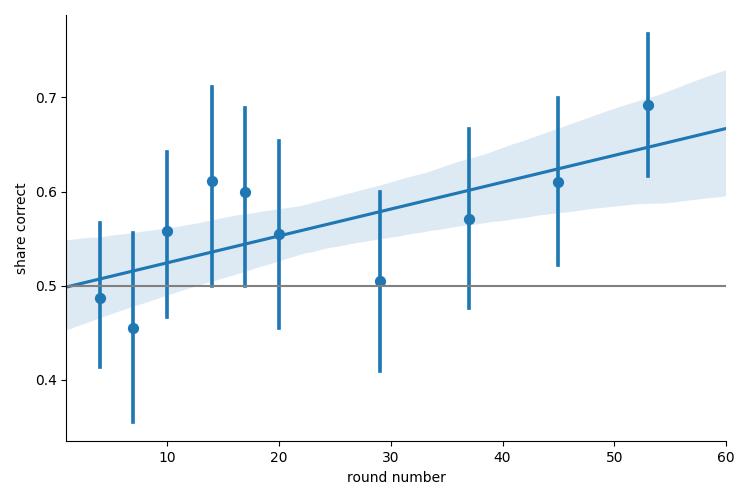
\includegraphics[width=0.5\linewidth]{../computed_objects/figures/learning_all} 

}

\caption{\label{learningAll} Share of correct predictions across rounds}\label{fig:learningAll}
\end{figure}

\hypertarget{conclusion}{%
\section{Conclusion}\label{conclusion}}

\renewcommand\refname{Appendix}
  \bibliography{bibliography.bib}

\end{document}
